
This section details an example integration of the \COP with
the open source PicoRV32 RISC-V core.

The example integration consists of a single PicoRV32 and \COP
connected via the Pico Co-Processor Interface (PCPI).

The PCPI is a feature of the PicoRV32.
We include the glue logic required in order to interface with the \COP.

The resulting sub-system has two memory ports, one for the \COP and one
for the PicoRV32.
Both memory ports are configured as AXI4-Lite interfaces.

\subsection{Sub-System Overview}

Figure \ref{fig:integration-block} shows the main ports and connections in
the example integration.

\begin{figure}[h]
\centering
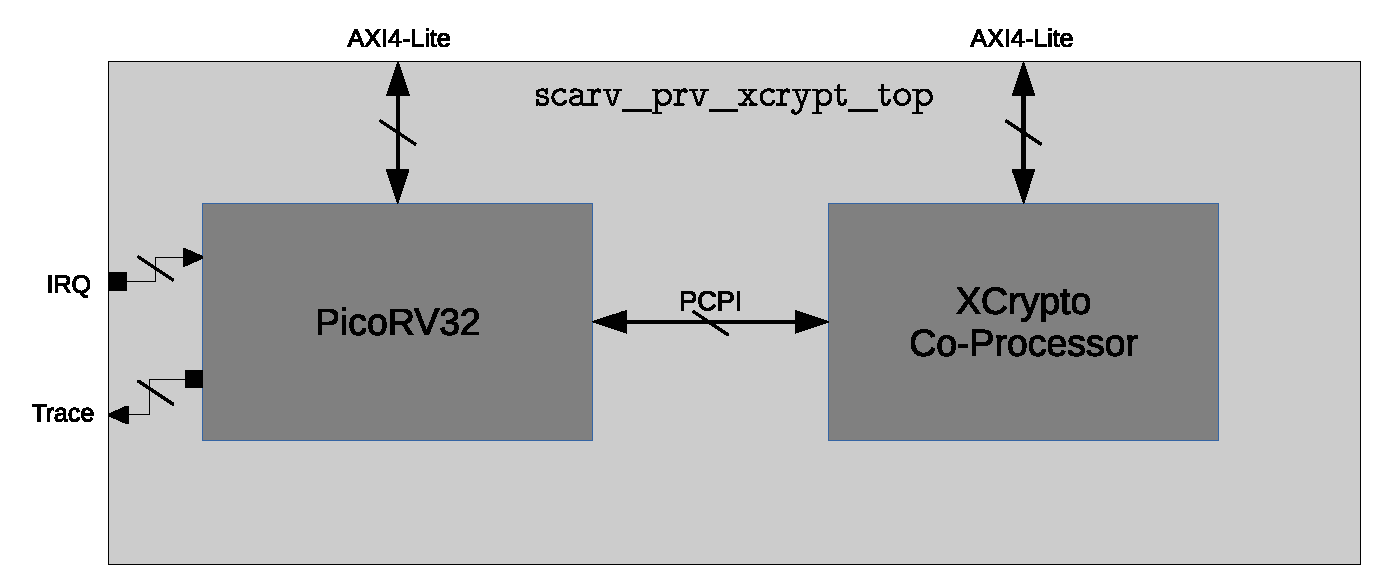
\includegraphics[width=1.0\textwidth]{diagrams/integration-block-diagram.eps}
\caption{Block diagram of the example \COP integration with the PicoRV32}
\label{fig:integration-block}
\end{figure}

The PicoRV32 memory, trace and interrupt interfaces are all exposed, along
with the \COP memory interface.

The top level module for the sub-system is {\tt scarv\_prv\_xcrypt\_top}.


\subsection{Integration Files}

This section lists the files required for working with the example
integration.

... TBD ...
